%-------------------------------------------------------------------------------
% HAWC data format manual
%-------------------------------------------------------------------------------

\documentclass[10pt,letter]{article}
\usepackage[titletoc,title]{appendix}
\usepackage{natbib}
%\usepackage{biblatex}
%\bibliography{enestmemo.bib}

% Line numbering
%\usepackage{lineno}
%\linenumbers

\usepackage{amsmath}
\usepackage{longtable}
\usepackage{url}
\usepackage[margin=1.5in]{geometry}
\usepackage{listings}
\lstset{frame=tb,
  language=C++,
  aboveskip=3mm,
  belowskip=3mm,
  showstringspaces=false,
  columns=flexible,
  basicstyle={\small\ttfamily},
  numbers=none,
  numberstyle=\tiny\color{gray},
  keywordstyle=\color{blue},
  commentstyle=\color{dkgreen},
  stringstyle=\color{black},
  breaklines=true,
  breakatwhitespace=true,
  tabsize=3
}
\usepackage{afterpage}
\usepackage[utf8]{inputenc}
\usepackage[english]{babel}
\usepackage[english]{isodate}
\usepackage[parfill]{parskip}
\usepackage[export]{adjustbox}
\usepackage{multirow}
\usepackage{graphicx}
\usepackage{enumitem}
\usepackage{rotating}
\usepackage[table]{xcolor}
\usepackage{caption}
\usepackage{listings}
\usepackage{subcaption}


\usepackage{float}
%\floatstyle{boxed}
\restylefloat{figure}

\usepackage{hyperref}
\definecolor{codegreen}{rgb}{0,0.6,0}
\definecolor{codegray}{rgb}{0.5,0.5,0.5}
\definecolor{codepurple}{rgb}{0.58,0,0.82}
\definecolor{backcolour}{rgb}{0.95,0.95,0.92}

\lstdefinestyle{mystyle}{
    backgroundcolor=\color{backcolour},   
    commentstyle=\color{codegreen},
    keywordstyle=\color{magenta},
    numberstyle=\tiny\color{codegray},
    stringstyle=\color{codepurple},
    basicstyle=\ttfamily\footnotesize,
    breakatwhitespace=false,         
    breaklines=true,                 
    captionpos=b,                    
    keepspaces=true,                 
    numbers=none,                    
    numbersep=5pt,                  
    showspaces=false,                
    showstringspaces=false,
    showtabs=false,                  
    tabsize=2
}

\lstset{style=mystyle}
\lstdefinestyle{filepath}{
  basicstyle=\ttfamily\small,
  breaklines=true,
  columns=fullflexible,
  breakindent=0pt
}
\captionsetup[table]{skip=1pt}



\hypersetup{
  colorlinks=true,
  linkcolor=blue,
  citecolor=blue,
  urlcolor=blue,
}

\newcommand{\specialcell}[2][c]{%
\begin{tabular}[#1]{@{}l@{}}#2\end{tabular}}

\newcommand*{\plogo}{%

\includegraphics[width=0.2\textwidth]{HAWCLogo.pdf}%
}%

\newcommand{\bi}{\begin{itemize}}
\newcommand{\ei}{\end{itemize}}
\newcommand{\be}{\begin{enumerate}}
\newcommand{\ee}{\end{enumerate}}
\newcommand{\tofix}[1]{{\color{red}#1}}

\addtolength{\textwidth}{3.5cm}
\addtolength{\oddsidemargin}{-2cm}
\addtolength{\topmargin}{-1cm}
\addtolength{\textheight}{3cm}


%----------------------------------------------------------------------------------------
%	TITLE PAGE
%----------------------------------------------------------------------------------------

\newcommand*{\titleGP}{\begingroup
\plogo

\centering
\vspace*{\baselineskip}



{\LARGE Technical Note: Time Dependent Analysis of HESS J0632+057}\\[0.4\baselineskip]

\rule{\textwidth}{0.4pt}\vspace*{-\baselineskip}\vspace{3.2pt}
\rule{\textwidth}{1.6pt}\\[\baselineskip]

{Junho Gyeong, Minji Shin and Chang Dong Rho \\ Sungkyunkwan University (SKKU)}
\\[\baselineskip]
\today  \par
\endgroup}







\begin{document}

% Title page stuff
\titleGP

\tableofcontents
\newpage

\section{Introduction} 
text goes here 


\section{Data} 
We use approximately 2886 days of HAWC data. The Pass 5 Final NN map with ML cut is used. The analysis bins are selected based on the recomended binning scheme for the declination of HESS J0632+057.
The maptree, detector response file, and the bin list used in this analysis are listed below.
\begin{itemize}[itemsep=0.1em]
    \item Maptree file:
    \begin{lstlisting}[style=filepath]
/lustre/hawcz01/hawcroot/maps/pass-5.final/Pass5-Final-ML-Map/pass5f-fhit2pct-chunk0001-1510-ML/maptree-fhit2pct-pass5f-mlp-chunk1-1510.root
    \end{lstlisting}
    \vspace{-0.5em}
    \item Detector response file:
    \begin{lstlisting}[style=filepath]
/lustre/hawcz01/hawcroot/maps/pass-5.final/Pass5-Final-ML-Map/pass5f-fhit2pct-chunk0001-1510-ML/detRes-fhit2pct-pass5f-mlp-refit.root
    \end{lstlisting}
    \vspace{-0.5em}
    \item Bin list:
    \begin{lstlisting}[style=filepath]
B0C0Ea B0C0Eb B0C0Ec B0C0Ed B0C0Ee B1C0Ea B1C0Eb B1C0Ec B1C0Ed B1C0Ee B2C0Ea B2C0Eb B2C0Ec B2C0Ed B2C0Ee B3C0Ea B3C0Eb B3C0Ec B3C0Ed B3C0Ee B3C0Ef B4C0Eb B4C0Ec B4C0Ed B4C0Ee B4C0Ef B5C0Ec B5C0Ed B5C0Ee B5C0Ef B5C0Eg B6C0Ed B6C0Ee B6C0Ef B6C0Eg B6C0Eh B7C0Ee B7C0Ef B7C0Eg B7C0Eh B7C0Ei B8C0Ee B8C0Ef B8C0Eg B8C0Eh B8C0Ei B8C0Ej B9C0Ef B9C0Eg B9C0Eh B9C0Ei B9C0Ej B10C0Eg B10C0Eh B10C0Ei B10C0Ej B10C0Ek B10C0El
    \end{lstlisting}
\end{itemize}
\section{Map-making} 
To study the orbital-phase dependence of HESS J0632+057, we divide the HAWC data into four orbital-phase intervals based on previous IACT and X-ray observations. We adopt an orbital period of 317 days and define phase zero as MJD 54857.0, corresponding to the date of the first Swift-XRT observation.
The four orbital states are defined as 

\begin{itemize}
    \item First high state:
    $\phi = 0.2$--$0.4$,

    \item Low state:
    $\phi = 0.4$--$0.6$,

    \item Second high state:
    $\phi = 0.6$--$0.8$,

    \item Medium state:
    $\phi = 0.8$--$0.2$.
\end{itemize}


\subsection{Map-making Procedure}
The reconstructed HAWC data, namely reduced dataset, are stored in individual chunks. We divide the Pass 5 reduced dataset according to the orbital phase of HESS J0632+057. Chunks 1-102 are excluded due to poor agreement between data and Monte Carlo simulations. After applying the phase selections, raw maps are generated separately for each chunk. Each reduced data file contains reconstructed event information, including the shower direction, core position, GPS time, and other event-level quantities. These quantities are used to assign the selected events to the corresponding pixels of the skymap. The Pass 5 binning scheme is applied during this step, resulting in a separate raw map for each bin. Because of computational and constraints, the raw maps are generated separately for individual chunks. The chunks-level raw maps are subsequently combined for each orbital state and Pass 5 bin to construct the phase-folded maps. After the chunk-level maps are combined, two additional process are applied: randomized background estimation and rejiggering.
The randomized background procedure is applied ti the high-energy bins, where limited event statistics can lead to unstable background estimates with the standard direct integration method. The final step is rejiggering, which smooths the background map on an angular scale of $0.5^\circ$. All scripts used for the map-making procedure can be found here: \href{https://gitlab.com/hawc-observatory/sandboxes/kyoungjh}{\texttt{map-making codes}}

\subsection{Sanity Check with Crab}
As a sanity check, we analyze the Crab Nebula in each phase-folded map. The Crab Nebula provides a stable reference source for validating the map-making procedure. It is modeled as a point source with a log parabola spectrum. Figure~\ref{fig:crab_sed} shows the SED of the Crab Nebula, and Table~\ref{tab:crab_fit} summarizes the best-fit spectral parameters obtained from each phase-folded map and the combined map. The best-fit spectral parameters are consistent among the phase-folded maps within their uncertainties. The corresponding TS values are also consistent with the different exposure times of the individual maps.

\begin{figure}[H]
    \centering
    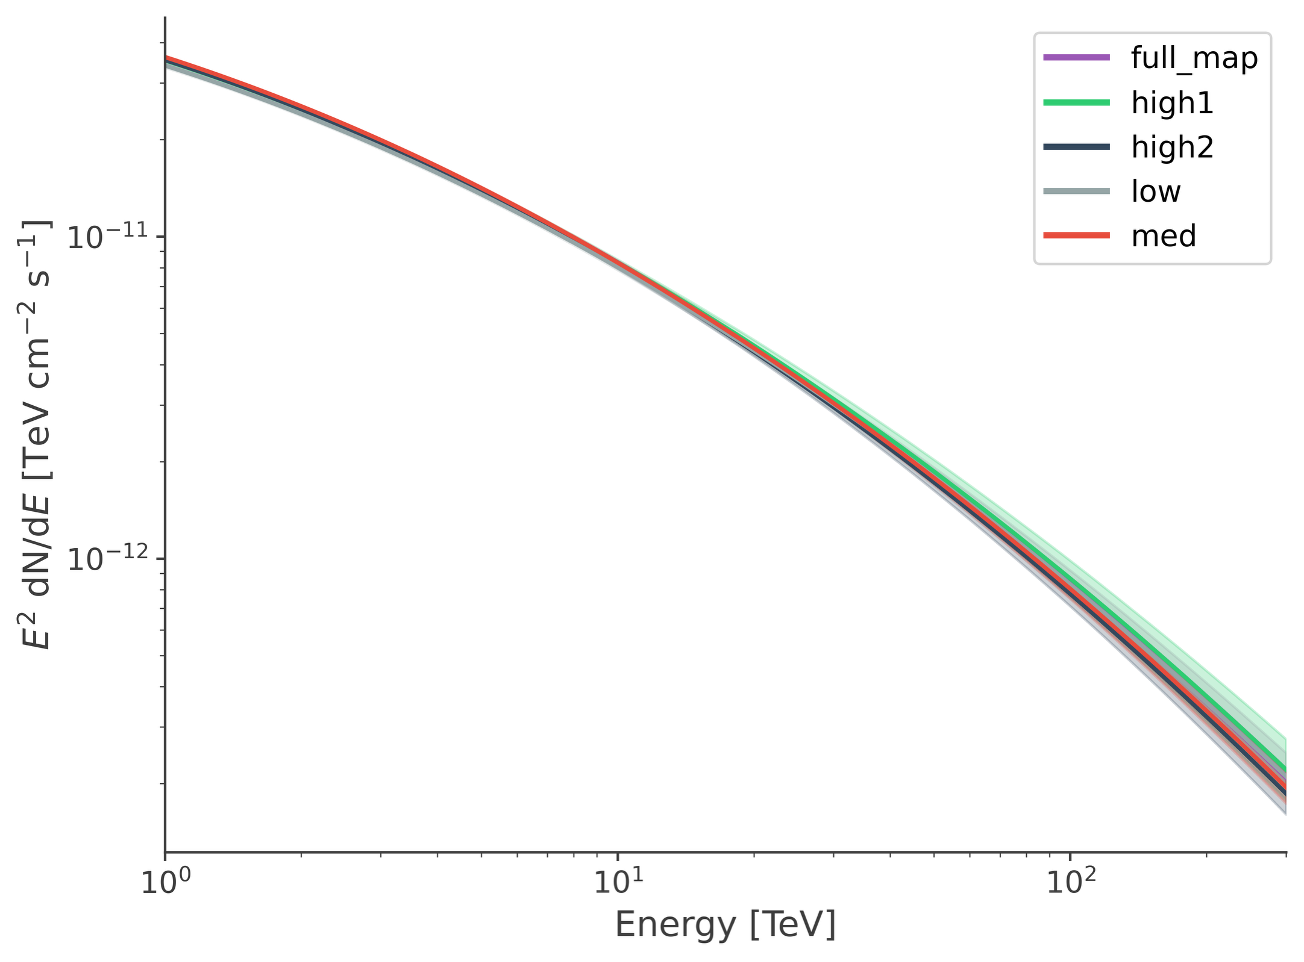
\includegraphics[width=0.8\textwidth]{Plots/Crab/Crab_SED.png}
    \caption{
    Spectral energy distributions of the Crab Nebula obtained from
    the combined map and the four phase-folded maps.
    }
    \label{fig:crab_sed}
\end{figure}


\begin{table}[H]
\centering
\caption{
Best-fit spectral parameters of the Crab Nebula obtained from the combined and phase-folded maps.
}
\label{tab:crab_fit}
\begin{tabular}{l|c|c|c|c|c}
\hline
Phase & Transits & K & $\alpha$ & $\beta$ & TS \\
\hline
Combined    & 2886.62 & {2.250 +/- 0.016} & {-2.758 +/- 0.008} & {0.079 +/- 0.003} & 95081.89 \\
First high & 521.927 & {2.27 +/- 0.04} & {-2.746 +/- 0.014} & {0.075 +/- 0.06} & 17348.49 \\
Low         & 575.175 & {2.16 +/- 0.04} & {-2.750 +/- 0.018} & {0.077 +/- 0.008} & 17822.27 \\
Second high & 595.732 & {2.21 +/-0.04} & {-2.772 +/- 0.018} & {0.082 +/- 0.008} & 19238.42 \\
Medium      & {1189.66} & {2.251 -0.026 +0.025} & {-2.773 +/- 0.013} & {0.080 +/- 0.005} & 39435.95 \\
\hline
\end{tabular}
\end{table}


\section{Baseline Modeling} 
The baseline modeling is performed using the combined map. We adopt a circular region of interest (ROI) with a radius of $3^\circ$, centered on the position of HESS J0632+057. The baseline analysis consists of two main steps: a systematic source search pipeline, followed by morphological and spectral modeling. Figure~\ref{fig:Combined_sigmap} shows the ROI.

\begin{figure}[H]
    \centering
    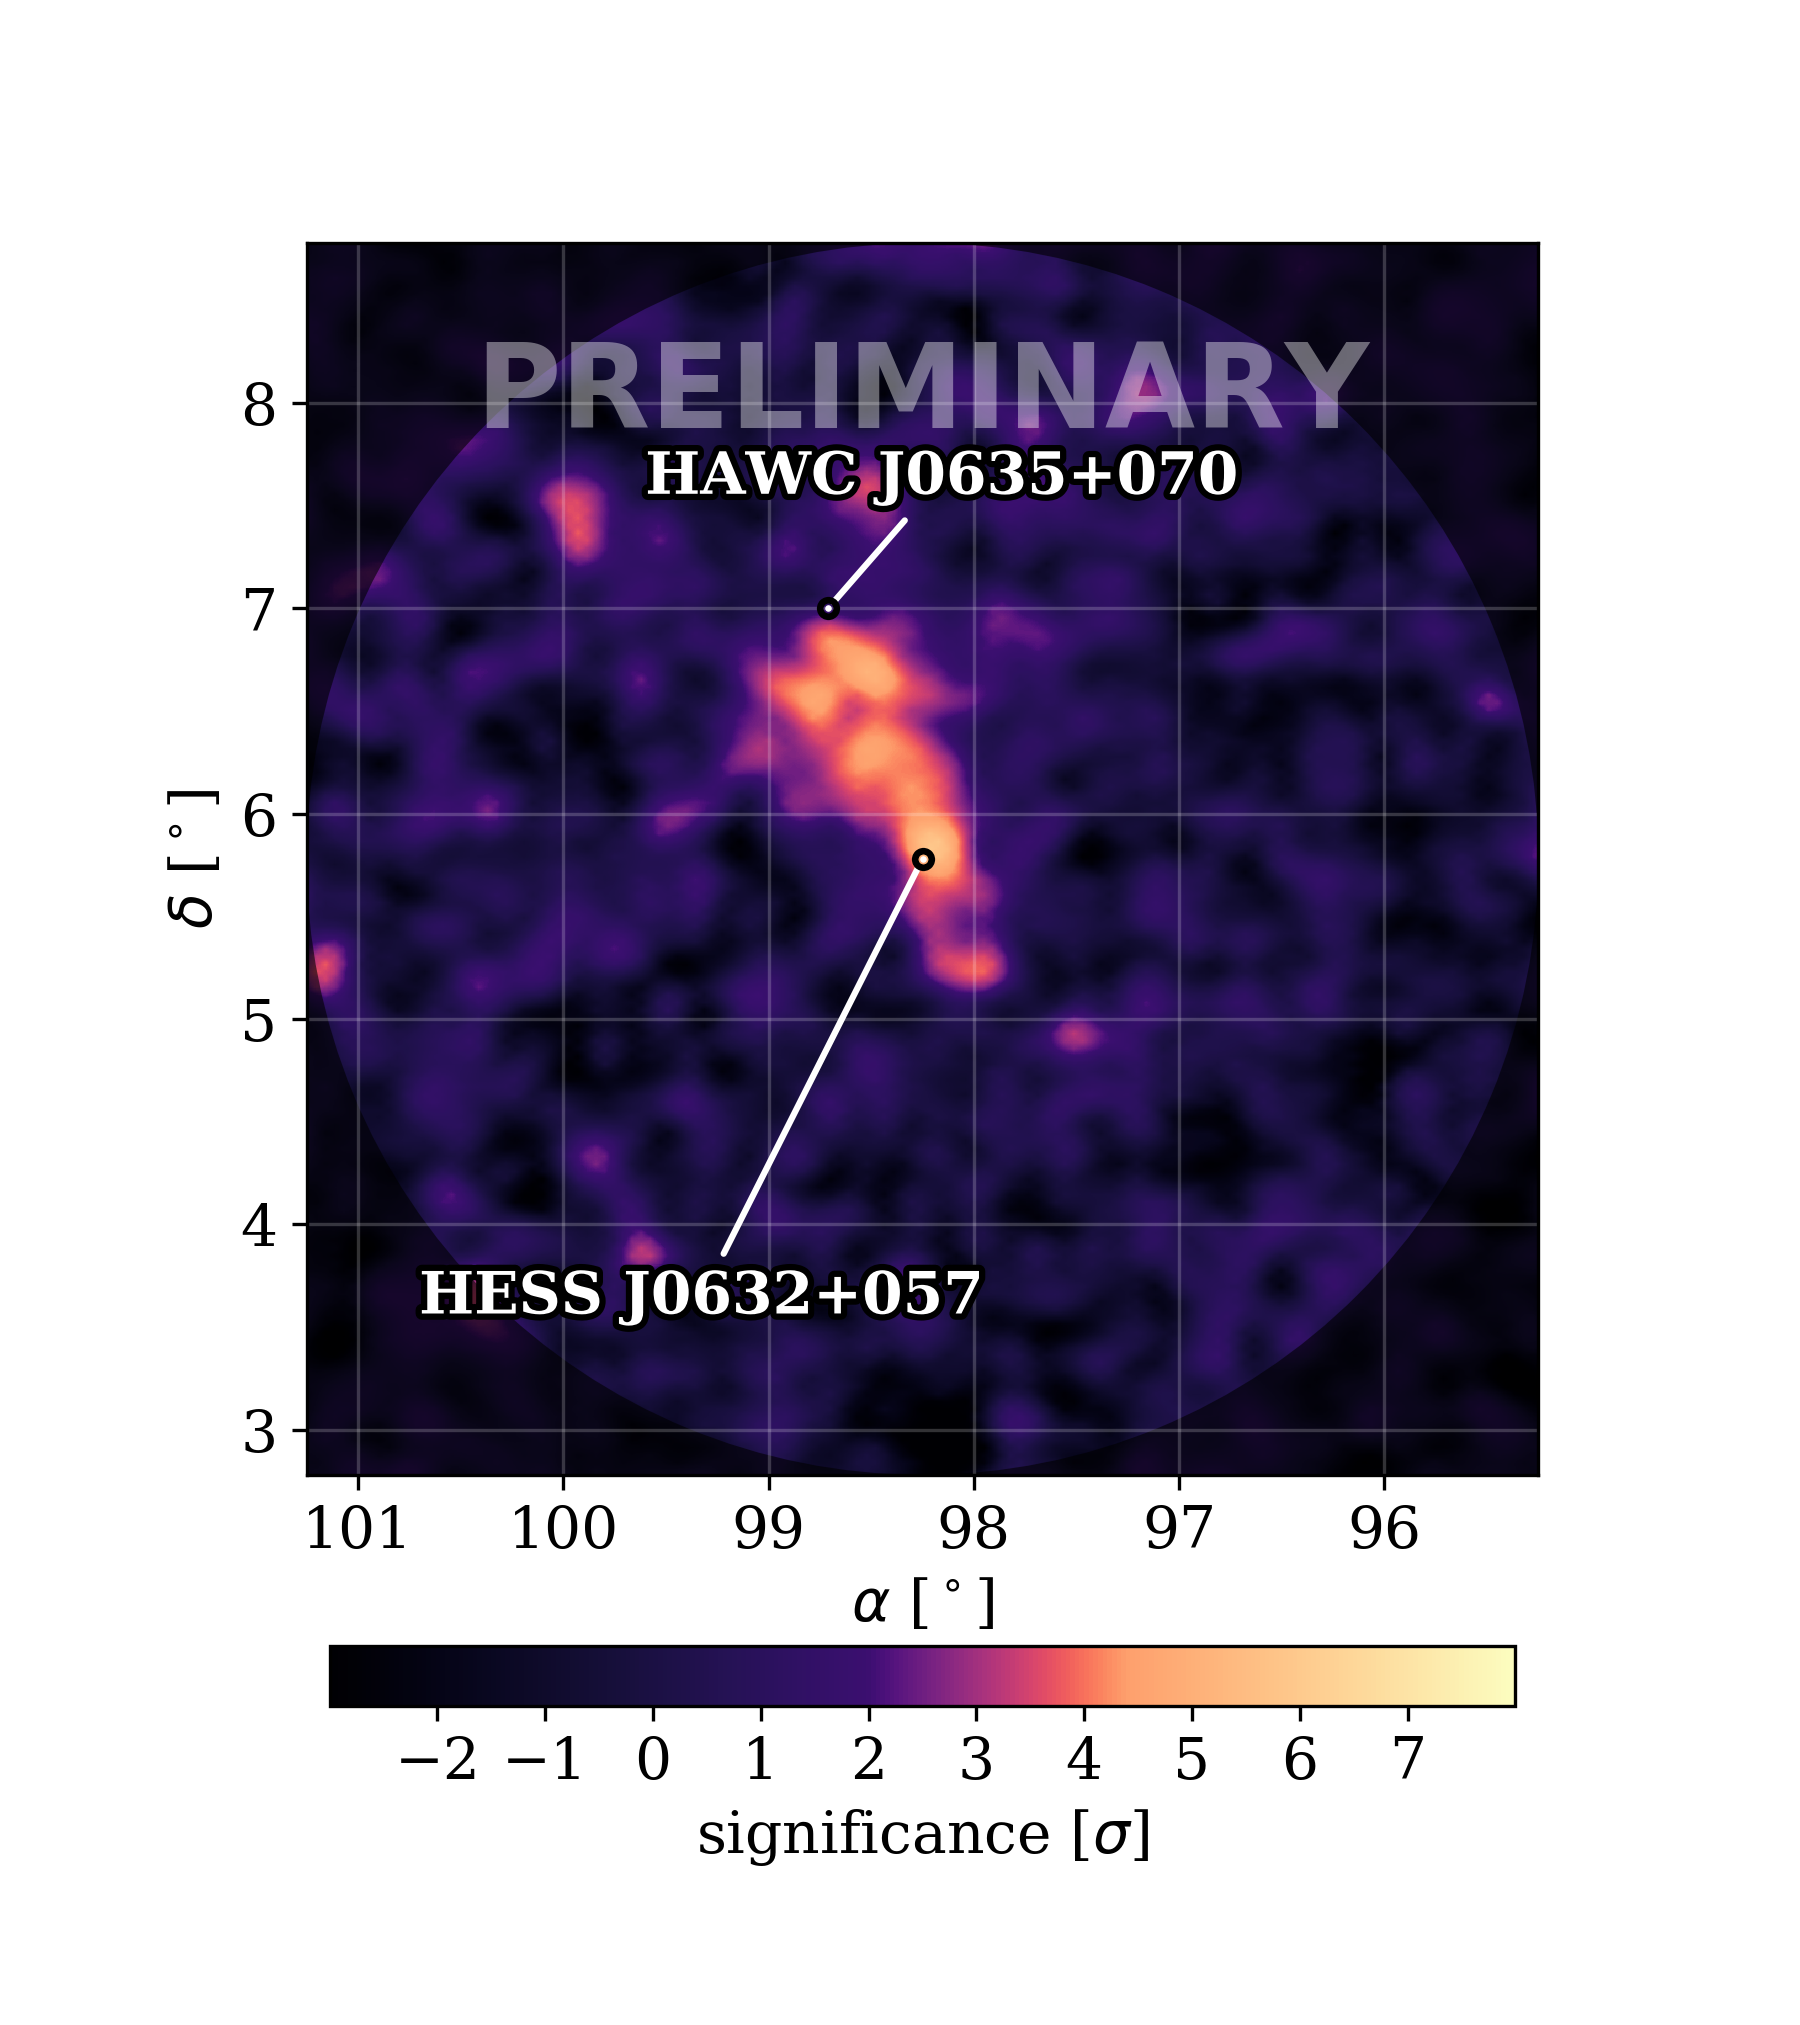
\includegraphics[width=0.8\textwidth]{Plots/Sigmap/combined_sigMap.png}
    \caption{
    caption
    }
    \label{fig:Combined_sigmap}
\end{figure}


\subsection{Systematic Source Search}
\subsection{Morphological and Spectral Modeling}
After identifying candidate sources with the systematic source-search
pipeline, we perform morphological and spectral modeling for Sources 1
and 2, which are associated with HESS J0632+057 and HAWC J0635+070,
respectively.

The morphological and spectral models tested for the two sources are
summarized in Table~\ref{tab:tested_models}. HESS J0632+057 is modeled
as a point source, while both Gaussian on the sphere and continuous
injection diffusion morphologies are tested for HAWC J0635+070.
For each morphology, power law, cutoff power law, and log parabola
spectral models are considered.
\begin{table}[H]
\centering
\caption{Morphological and spectral models tested for HESS J0632+057
and HAWC J0635+070.}
\label{tab:tested_models}
\renewcommand{\arraystretch}{1.3}
\begin{tabular}{c|c|c}
\hline
\textbf{Source} & \textbf{Morphology} & \textbf{Spectrum} \\
\hline

\multirow{3}{*}{HESS J0632+057}
& \multirow{3}{*}{Point source}
& Power law \\
& & Cutoff power law \\
& & Log parabola \\
\hline

\multirow{6}{*}{HAWC J0635+070}
& \multirow{3}{*}{Gaussian on the sphere}
& Power law \\
& & Cutoff power law \\
& & Log parabola \\
\cline{2-3}

& \multirow{3}{*}{Continuous injection diffusion}
& Power law \\
& & Cutoff power law \\
& & Log parabola \\
\hline
\end{tabular}
\end{table}

The results of the model comparison are summarized in
Table~\ref{tab:model_comparison}. Considering the likelihood improvement together with the additional degrees of freedom introduced by more complex spectral models, we adopt a point source with a powerlaw spectrum for HESS J0632+057 and a continuous injection diffusion morphology with a cutoff powerlaw spectrum for HAWC J0635+070 as the baseline model.

For HESS J0632+057, the cutoff powerlaw model provides an improvement in the likelihood compared with the simple power-law model. However, the improvement is not sufficient to justify the additional spectral parameter, and the simpler powerlaw model is therefore adopted for the baseline analysis.

\begin{table}[H]
\centering
\caption{Comparison of the model combinations for HESS J0632+057 and HAWC J0635+070.}
\label{tab:model_comparison}

\resizebox{\textwidth}{!}{
\begin{tabular}{c|c|c|c|c|c|c}
\hline
\multicolumn{2}{c|}{\textbf{HESS J0632+057}} &
\multicolumn{2}{c|}{\textbf{HAWC J0635+070}} &
\multirow{2}{*}{\textbf{$-\log L$}} &
\multirow{2}{*}{\textbf{AIC}} &
\multirow{2}{*}{\textbf{BIC}} \\
\cline{1-4}
Morphology & Spectrum & Morphology & Spectrum & & & \\
\hline

\multirow{18}{*}{Point source}

& \multirow{6}{*}{Power law}
& \multirow{3}{*}{Gaussian on the sphere}
& Power law        & 107516.27 & 215050.53 & 215156.47 \\
& & & Cutoff power law & 107510.04 & 215040.09 & 215157.81 \\
& & & Log parabola      & 107511.47 & 215042.94 & 215160.65 \\

\cline{3-7}

& & \multirow{3}{*}{Continuous injection diffusion}
& Power law & 107514.34 & 215046.68 & 215152.62 \\
& & & \textbf{Cutoff power law} & \textbf{107508.37} & \textbf{215036.74} & \textbf{215154.46} \\
& & & Log parabola & 107510.07 & 215040.14 & 215157.86 \\

\cline{2-7}

& \multirow{6}{*}{Cutoff power law}
& \multirow{3}{*}{Gaussian on the sphere}
& Power law & 107521.19 & 215062.39 & 215180.10 \\
& & & Cutoff power law & 107509.72 & 215041.45 & 215170.93 \\
& & & Log parabola & 107511.16 & 215044.32 & 215173.80 \\

\cline{3-7}

& & \multirow{3}{*}{Continuous injection diffusion}
& Power law & 107520.49 & 215060.99 & 215178.70 \\
& & & Cutoff power law & 107507.96 & 215037.93 & 215167.42 \\
& & & Log parabola & 107509.75 & 215041.50 & 215170.99 \\

\cline{2-7}

& \multirow{6}{*}{Log parabola}
& \multirow{3}{*}{Gaussian on the sphere}
& Power law & 107516.02 & 215052.04 & 215169.75 \\
& & & Cutoff power law & 107510.05 & 215042.10 & 215171.59 \\
& & & Log parabola & 107511.46 & 215044.93 & 215174.41 \\

\cline{3-7}

& & \multirow{3}{*}{Continuous injection diffusion}
& Power law & 107513.75 & 215047.50 & 215165.21 \\
& & & Cutoff power law & 107508.33 & 215038.65 & 215168.14 \\
& & & Log parabola & 107510.06 & 215042.12 & 215171.61 \\

\hline
\end{tabular}
}

\end{table}

Figure~\ref{fig:baseline_sed} shows the resulting spectral energy
distribution and energy-dependent emission obtained with the baseline
model.




\section{Phase-dependent Analysis}
The baseline source model derived from the combined map is used as the starting point for the phase-dependent analysis. The four phase-folded maps corresponding to the first high, low, second high, and medium states are analyzed separately. Figure~\ref{tab:Sgi_map_phase_folded} shows the pre-trial significance maps for each orbital state. 
The spectral properties of HESS J0632+057 are then compared among the four orbital states to investigate possible orbital modulation of the VHE gamma-ray emission.
In the phase-dependent analysis, the spectral and morphological parameters of HAWC J0635+070 are fixed to the best-fit values obtained from the combined map. Since the phase-folded maps are constructed according to the orbital phase of HESS J0632+057, HAWC J0635+070 is assumed to remain unchanged among the four orbital states. In addition, the morphological parameters of HESS J0632+057 are fixed to the values obtained from the combined-map analysis because of the limited statistics in the individual phase-folded maps.
Table~\ref{tab:best-fit_result_phase_folded} summarizes the best-fit results for each orbital state. Figure~\ref{tab:residual_map_phase_folded} shows the corresponding model and residual maps, together with the one-dimensional significance distributions.
Enhanced gamma-ray flux is observed during the two high states, while the flux decreases during the low state. This behavior is consistent with the orbital flux variability previously observed by IACTs. The best-fit gamma-ray indices range from approximately 2.8 to 3.4 among the four orbital states. 
Figure X~\ref{tab:SED_phase_folded} shows the SED of HESS J0632+057 for the four orbital states and compares the HAWC measurements with previous IACT results.

\section{Discussions} 

\section{Systematic studies} 
text goes here
%\section{Systematic Uncertainties} 

\section{References} 
text goes here
\end{document}